
\begin{frame}[t,allowframebreaks]{Regularisation -}

The `no free lunch' theorem of \gls{ml} implies that we
need to design our algorithms 
to perform well on \underline{specific tasks}.

\vspace{0.2cm}

We do this, for example, by:
\begin{itemize}
    \item adjusting the algorithm's 
    \index{representational capacity}\gls{representational capacity}, or by    
    \item giving an algorithm a 
    {\bf preference for some type of solution}.
\end{itemize}

\vspace{0.2cm}

Several known {\bf strategies to reduce the test/generalisation error},
possibly at the price of increasing the training error,
are {\bf referred to collectively as
\index{regularisation}\gls{regularisation}}.

{\color{red} \tiny
We can prescribe preferences by adding a 
\index{regularisation}\index{regulariser}\gls{regulariser} to the 
\index{cost function}\gls{cost function}.

\begin{itemize}
 \item A \gls{regulariser} penalises the choice of non-preferred solutions.
 \item Non-preferred solutions are still eligible and 
 can one can be chosen if it fits the training data significantly 
 better than the preferred solution.
\end{itemize}
}


\framebreak

%
%

A simple form of \index{regularisation}\gls{regularisation} is 
\index{weight decay}\gls{weight decay}.\\
\vspace{0.2cm}

We can modify the loss function, $L(\vect{w})$, 
to include a \index{regulariser}\gls{regulariser} $\Omega(\vect{w})$:
\begin{equation}
    L(\vect{w}) \rightarrow L(\vect{w}) + \Omega(\vect{w})
    %\label{eq:}
\end{equation}\\

The \gls{regulariser} has the form:
\begin{equation}
    \Omega(\vect{w}) = \lambda \vect{w}^T \vect{w} 
    %\label{eq:}
\end{equation}\\

and expresses a {\bf preference for the weights to have a smaller $L^2$ norm}.
The factor $\lambda$ is fixed prior to training and controls the
strength of our preference for smaller weights.
\vspace{0.2cm}

Minimising $L(\vect{w})$ results in a tradeoff, 
in the choice of $\vect{w}$, between:
\begin{itemize}
\item fitting the training data, and
\item being small.
\end{itemize}

\framebreak

%
%

Using $\Omega(\vect{w})$, we can now control 
a model's tendency to overfit or underfit.\\
\vspace{0.2cm}
{\small
The following example, shows the impact of different values of $\lambda$ 
on the result of training a high-degree (degree 9) polynomial regression model
to examples from a quadratic data-generating distribution.\\
}

\begin{columns}
    \begin{column}{0.65\textwidth}
        \begin{center}
            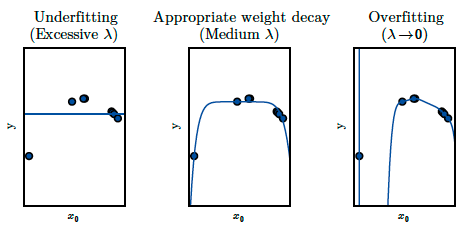
\includegraphics[width=0.99\textwidth]
                {./images/training_issues/goodfellow17_regularisation_weigh_decay_example_1.png}\\
            {\tiny 
                Using weight decay to control a model's tendency to overfit or underfit.\\
                \color{col:attribution} 
                Schematic reproduced from p. 116 of \cite{Goodfellow:2017MITDL}.\\
            }
        \end{center}        
    \end{column}
    \begin{column}{0.35\textwidth}
    \end{column}
\end{columns}

\end{frame}